\documentclass[a4paper]{memoir}
\usepackage[utf8]{inputenc}
\usepackage[frenchb]{babel}
\usepackage{graphicx}
\usepackage{float}
\usepackage{hyperref}
\usepackage{verbatim}
\usepackage{enumitem}
\usepackage[babel=true]{csquotes}

\pagestyle{plain}

\title{
	\textbf{Rapport de projet}
	\bigskip
	\begin{center}
		
\includegraphics[scale=0.25]{img/OpenSculpt.png}
	\end{center}
	\bigskip
}
\author{\emph{GAUTHIER Silvère}\\\emph{LAMEIRA Yannick}\\\emph{PELADAN Cécile}}
\date{\today}

\begin{document}
	\maketitle
	\newpage
	\tableofcontents

	\chapter{Remerciements}

		Un grand merci à Frédéric Boudon et Benjamin Gilles pour leur encadrement.
		Un remerciement particulier à Frédéric Boudon pour son idée d'outil de subdivision locale.

	\chapter{Introduction}
		
		\section{Sujet initial}
			L'objectif de ce projet est de créer un logiciel de sculpture 3D. L'utilisateur aurait à disposition un maillage déformable, qu'il pourrait 
			modeler avec différents outils tels que déplacement, ajout de matière ou lissage. L'interface devra permettre à l'utilisateur de facilement 
			créer un maillage initial, le visualiser et interagir avec lui à l'aide des différents outils de modelage. Initialement, les premières 
			fonctionnalités à implémenter seront la création d'une sphère ou d'un cube comme maillage de départ, la navigation dans l'espace 3D pour se 
			positionner autour du maillage, puis les outils de déformation cités ci-dessus. Une interface graphique contenant les boutons d'outils sera 
			définie pour que l'utilisateur puisse intuitivement appliquer les différentes opérations proposées.

			Les principales difficultés ici seront d'abord de gérer correctement l'interaction 3D de l'utilisateur avec le maillage via le curseur et la 
			fenêtre 2D. Ensuite viendra la mise en place d'une structure de données efficace et robuste de maillage avec l'implémentation des algorithmes 
			de subdivision et de raffinement.

			Si le temps le permet, d'autres outils et maillages de base pourront être implémentés, afin d'enrichir le logiciel. On pourra également 
			réfléchir à une manière d'importer et exporter les maillages sous différents formats tels que le OBJ ou le STL par exemple.

			Ce logiciel sera développé en C++ avec la bibliothèque OpenGL pour le rendu 3D et la bibliothèque Qt pour définir l'interface.

%==========================================================================================================================================================
	\chapter{Cahier des charges}
		Ce chapitre détaille la phase de conception du projet.
			
		\section{Mécanismes}
			Cette section détaille succintement les fonctionnalités de l'application.
			
			\subsection{Les Modèles}
				\label{model-cdc}
				Différents maillages prédéfinis, appelés ici modèles, seront mis à disposition de l'utilisateur.\\
				Nous en prévoyons actuellement cinq, paramétrables par l'utilisateur :
				\begin{itemize}
					\item \textbf{Cube :} défini par une largeur, une hauteur et une profondeur.
					\item \textbf{Sphère :} défini par un rayon.
					\item \textbf{Cylindre :} défini par une hauteur et un rayon.
					\item \textbf{Cône :} défini par une hauteur et un rayon.
					\item \textbf{Tore :} défini par un rayon horizontal et un rayon vertical.
				\end{itemize}
				Chaque modèle sera aussi paramétré par un pas de discrétisation.
				
			\subsection{Le Rendu}
				Le rendu s'effectuera dans une classe spécifique, et permet de synchroniser la structure interne des maillages avec les buffer objects. Il 
				existera également différentes options de rendu telles que l'affichage solide ou en fils de fer, les couleurs, les lumières...etc.

			\subsection{Les Outils de sculpture}
				\label{tool-cdc}
				Différents outils seront disponibles. Ils auront pour action de modifier le maillage dans la direction des normales de surface, et selon
				un schéma de modification propre à chaque outil. Nous avons défini deux catégories d'outils : modifications globales et locales des objets
				(une troisième est destinée au déplacement de la caméra dans la scène en trois dimensions).
				\newpage
				\begin{itemize}
					\item \textbf{Modifications Globales :}
					\begin{itemize}
						\item \textbf{GTMove :} Déplacement d'un objet dans le repère scène.
						\item \textbf{GTRotate :} Rotation d'un objet dans le repère scène.
						\item \textbf{GTScale :} Mise à l'échelle d'un objet dans le repère scène.
					\end{itemize}
					\item \textbf{Modifications Locales :}
					\begin{itemize}
						\item \textbf{LTAdd :} Ajout de matière à la surface de l'objet.
						\item \textbf{LTSmooth :} Lissage de la surface de l'objet.
						\item \textbf{LTMove :} Déplacement d'une partie des points de la surface de l'objet.
						\item \textbf{LTInflate :} Gonflement de la surface de l'objet.
						\item \textbf{LTPinch :} Pincement de la surface de l'objet.
					\end{itemize}
				\end{itemize}
				Pour plus de détails sur leur fonctionnement, référez-vous à la partie \textbf{Développement} (cf page \pageref{tool-dev}).

			\subsection{Les Algorithmes de maillage}
				Les différents algorithmes de modification de maillages seront regroupés dans une classe statique spécifique. Y seront présentes les 
				fonctions de subdivision et de décimation globale, ainsi qu'une subdivision et une décimation automatique paramétrable avec une longueur 
				(maximale ou minimale) d'arête.

			\subsection{Interface}
				L'interface de l'application devra être ergonomique et proposer de nombreux raccourcis clavier afin de permettre à l'utilisateur de 
				travailler rapidement. Elle devra également être le plus intuitive possible, car un tel logiciel pourrait devenir très compliqué à 
				appréhender. Cela concernera tant les dispositions que les icônes qui devront suivre une certaine logique.

			\subsection{Les Options}
				% TODO : détailler brièvement les options de rendu, d'interface...etc
	
		\section{Structure du programme}
			Cette partie détaille succintement la structure globale du logiciel, ce qui couvre les aspects non maîtrisables par l'utilisateur.
			
			\subsection{L'API}
				L'application devra contenir une surcouche, ayant pour objectif de rendre notre logiciel facilement extensible par d'autres développeurs, 
				sans qu'ils aient besoin de connaître tous les détails de la structure interne de celui-ci.
				
				La structure interne des maillages retenue ici est la structure par demi-arêtes. Nous auront donc, pour chaque maillage, des listes de 
				points, faces et demi-arêtes.\\ Chaque point contiendra des coordonnées en trois dimensions, un indice de position dans la liste afin 
				d'améliorer la vitesse d'accès, ainsi qu'un pointeur vers une demi-arête sortante.\\ Chaque face contiendra un pointeur vers une demi-arête 
				intérieure, et éventuellement un vecteur normal.\\ Chaque demi-arête contiendra des pointeurs vers : une face, un point, les demi-arêtes 
				suivantes et précédentes au sein de la même face, et la demi-arête opposé.
				
				Plusieurs méthodes publiques devront être présentes, telles que "ajouter une face", "couper une arête en deux", "fusionner deux arêtes"... 
				et cacher la structure interne (n'agir qu'à l'aide de coordonnées par exemple). Cela permettra dans le futur, si besoin, de changer la 
				structure interne sans modifier le reste de l'application.
		
%==========================================================================================================================================================
	\chapter{Gestion du projet}
		Cette partie traite globalement de tout ce qui concerne l'organisation du projet, que ce soit au niveau de la conception, du développement, de 
		l'équipe ou encore de la gestion des fichiers.
		
		\section{Gestion de l'équipe}
			Tous les membres se connaissant et étant supposés être capable de travailler en équipe, nous n'avons fait aucune élection préalable de chef de 
			projet.\\ Mais le déroulement du projet nous a imposé ce choix, GAUTHIER Silvère assurera donc ce rôle, afin de garder une cohésion de groupe 
			et assurer la réalisation de nos objectifs.\\ Chaque membre peut tout de même participer activement au projet, autant lors de la conception que 
			du développement. Toutes les décisions seront prises suivant la majorité lors de votes.\\\\
			Pour ce qui est des réunions de projets, nous avons convenu avec nos tuteurs d'une réunion, allant d'environ trente minutes à une heure, toutes 
			les semaines, afin de mettre au point l'avancement du projet. En parallèle, tous les membres de notre équipe se retrouvent une fois par semaine 
			afin de discuter des points clés effectués ou à venir, donner lieu aux votes pour les prises de décisions, ou encore, lors de la phase de 
			développement, travailler en collaboration afin d'optimiser notre travail.\\\\
			Au niveau du travail collaboratif, nous avons mis en place un dépôt sur github (adresse à la page \pageref{url:github}), contenant tant la 
			documentation que les sources de notre programme. Par ailleurs, nous mettrons sur ce dépôt uniquement les fichiers sources et les images, mais 
			en aucun cas les fichiers temporaires ou les exécutables. Les seuls fichiers binaires disponibles seront les PDF de la documentation, pour un 
			soucis de facilité d'accès et de lecture.

		\section{Découpage en tâches}
			Afin de préparer le développement du programme, il était nécessaire de séparer les fonctionnalités les unes des autres. Nous avons abouti à ce 
			diagramme, qui résume notre choix de découpage :\\
			\begin{figure}[H]
				\begin{center}
					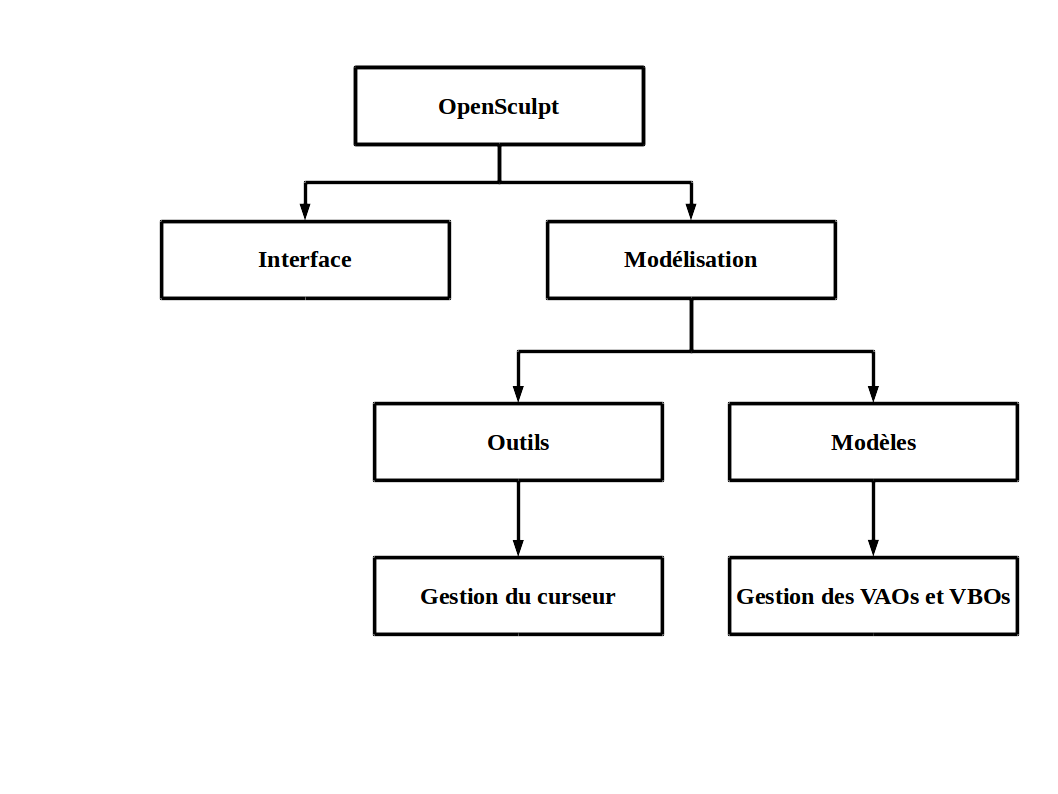
\includegraphics[scale=0.5]{img/DiagrammeDecoupageProjet.png}
				\end{center}
				\label{fig:decoupage}
				\caption{Diagramme des tâches du projet}
			\end{figure}

		\section{Assignation}
			Le projet étant découpé en un certain nombre de modules, il ne restait plus qu'à assigner chaque tâche à un ou plusieurs membres de l'équipe. 
			Nous nous sommes organisés comme ceci :
			\begin{itemize}[label=$\bullet$]
				\item \textbf{Conception, implémentation et vérifications de l'API} : GAUTHIER Silvère.
				\item \textbf{Mise en place de l'interface} : LAMEIRA Yannick.
				\item \textbf{Implémentation des maillages modèles} : PELADAN Cécile.
				\item \textbf{Conception et implémentation des outils} : GAUTHIER Silvère, LAMEIRA Yannick, PELADAN Cécile.
				\item \textbf{Tests et vérifications de l'application} : GAUTHIER Silvère, LAMEIRA Yannick, PELADAN Cécile.
			\end{itemize}
			Bien entendu, les membres pourront évidemment faire appel aux autres pour trouver une solution à un problème par exemple.\\
			Le détail complet des tâches et assignations se situe dans la section Gestion du temps, page \pageref{GestionTps}.

		\section{Gestion du temps}
			\label{GestionTps}
			Afin de clarifier notre gestion du temps, deux diagrammes de Gantt (prédictif et final) sont disponibles en annexe (cf page \pageref{fig:gantt}) 
			et dans la documentation de notre projet.\\

		\section{Choix technologiques}
			Afin de pouvoir développer correctement notre logiciel, il a fallu définir tout ce que nous allions utiliser en terme de langages et 
			bibliothèques selon notre logique de conception.
			
			\subsection{Langages de programmation}
				Pour des besoins de performances, nous avons comparé différents langages. Pour réduire le temps de recherche et de comparaison, nous nous 
				sommes appuyé sur des tests déjà effectués par d'autre.\\ Des tests de performances concernant un large panel de langages, comparés dans 
				quatre contextes différents, sont fournis en annexe, page \pageref{fig:analyse}.\\ Nous pouvons observer que globalement, le langage le plus 
				rapide est ici C++. L'utilisation de ce langage étant très fréquente dans les applications en temps réel, de part sa réputation d'un des 
				langages les plus performants, et tous les membres de notre équipe sachant l'utiliser, nous avons fait le choix de programmer le logiciel en 
				C++.\\

			\subsection{Bibliothèques}
				Pour la gestion graphique de l'interface et de l'affichage de l'objet, nous avons cherché une bibliothèque relativement simple d'utilisation 
				mais surtout performante afin de garder la fluidité gagnée avec le choix des langages de programmation.\\ Connaissant la bibliothèque 
				OpenGL, qui est bas niveau et performante dans les affichages deux et trois dimensions, nous nous sommes tournés vers une bibliothèque 
				utilisant OpenGL : Qt.\\

			\subsection{Représentation du maillage}
				Nous cherchons ici à comparer différentes techniques permettant de représenter un maillage, afin de choisir celle qui sera la plus adaptée à 
				nos opérations. Voici un tableau récapitulatif de cette étude comparative :
				\begin{table}[H]
					\begin{small}
						\hspace{-2,5cm}
						\begin{tabular}{| c | l | l |}
							\hline
							\textbf{Représentation} & \textbf{Avantages} & \textbf{Inconvénients}\\
							\hline
							 & - Hiérarchie des résolutions & - Visualisation surfacique difficile\\
							Octree ou KDTree & - Rendu volumique possible & - Coût de stockage excessif\\
							 & - Construction et parcours simples & - Recalculer à chaque modification\\
							\hline
							 & - Historique de construction & - Non unicité\\
							Arbre CSG & - Approche fonctionnelle & - Opérations complexes\\
							 &  & - Domaine insuffisant\\
							\hline
							G-maps & - Opérations de topologie simples & - Séparation topologie / plongement\\
							 & - Plongements multiples & \\
							\hline
							Liste de triangles & - Opérations simples & - Stockage non optimisé\\
							\hline
							Sommets partagés & - Opérations simples & \\
							 & - Stockage correct & \\
							\hline
							Bandes de triangles & - Stockage correct & - Chaque sommet est visité deux fois\\
							 &  & - Opérations de déplacement délicates\\
							\hline
							Structure par faces & - Chaque face pointe sur ses sommets & - Pas d'accès direct aux arêtes\\
							 & - Une face connaît les faces adjacentes & \\
							\hline
							Structure par demi-arêtes & - Parcours de maillage très pratiques & - Coût de stockage excessif\\
							\hline
							Vertex Array (VAO) & - Optimisé pour le rendu OpenGL & - Utilise le CPU et la RAM\\
							 & - Simple d'utilisation & \\
							\hline
							Vertex Buffer Object (VBO) & - Optimisé pour le rendu OpenGL & \\
							 & - Utilise le GPU et la VRAM & \\
							\hline
						\end{tabular}
					\end{small}
					\label{tab:maillage}
					\caption{Tableau comparatif de méthodes de représentation de maillage 3D}
				\end{table}
				L'étude comparative montre qu'il serait judicieux d'utiliser conjointement des Vertex Buffer Objects (VBOs) afin d'optimiser les 
				performances d'affichage et une classe personnalisée pour aisément gérer nos données par une surcouche de méthodes. La structure interne des 
				maillages sera donc une structure de type demi-arêtes, afin de faciliter les opérations de voisinage.
			
		\section{Gestion des fichiers}
			Nous avons beaucoup de fichiers à gérer dans ce projet, et nous devions établir des conventions ou des moyens afin de les gérer correctement.
			
			\subsection{Format des Fichiers}
				Le code étant écrit en C++, nous utiliserons des fichiers d'en-tête au format H et des fichiers de définition au format CPP.\\
				Toutes les images nécessaires au logiciel seront au format PNG afin de pouvoir utiliser la transparence et garder la pleine qualité d'image 
				(contrairement à JPEG qui perd de l'information à la compression).\\
			
				\subsubsection{Sauvegarde}
					Une façon judicieuse de sauvegarder nos données serait d'avoir un format spécial pour enregistrer un projet complet contenant une liste 
					d'objets, ainsi qu'une possibilité d'exportation de chaque objet ou scène dans un format connu tel que STL ou OBJ.
			
			\subsection{Commentaires}
				Si une méthode ou fonction (voir même un bloc) dépasse une certaine taille ou devient trop compliquée, un commentaire sera ajouté avant 
				celle-ci expliquant brièvement son processus :
				\begin{verbatim}
					/** Description :
					*** Entrée : ...
					*** Sortie : ...
					**/
				\end{verbatim}
				Quelque commentaires précieux pour le travail collaboratif seront également présents :
				\begin{table}[H]
					\begin{small}
						\hspace{-0,5cm}
						\begin{tabular}{| c | c |}
							\hline
							\textbf{Marqueur spécifique} & \textbf{Signification}\\
							\hline
							TODO & A mettre à la place du code d'une fonctionnalité à implémenter\\
							\hline
							RECODE & A mettre au dessus du bloc d'une fonctionnalité à refaire ou à optimiser\\
							\hline
							FIXME & A mettre au dessus du bloc d'une fonctionnalité contenant un bug\\
							\hline
						\end{tabular}
					\end{small}
					\label{tab:commentaire}
					\caption{Forme et usage des commentaires}
				\end{table}

			\subsection{Conventions de Nommage}
				Pour la lisibilité et la bonne pratique du développement de l'application, il est nécessaire de suivre des règles établies au sein de 
				l'équipe de projet, appelées conventions. Ainsi, nous avons choisi d'écrire le code en anglais uniquement, mis à part pour les commentaires 
				utiles aux développeurs préférant le français. De même, au moins une ligne de commentaire est requise avant chaque déclaration de classe ou 
				de fonction, afin d'en expliquer brièvement son fonctionnement (sauf dans le cas de méthodes simples avec des noms explicites).\\
				Voici un tableau récapitulatif des conventions de nommages pour les noms de variables, classes et méthodes :
				\begin{table}[H]
					\begin{small}
						\hspace{1,5cm}
						\begin{tabular}{| c | c |}
							\hline
							\textbf{Type de variable} & \textbf{Format du nom}\\
							\hline
							Classe & Majuscule suivit de minuscules\\
							\hline
							Méthode & Minuscules (pour les mots composés,\\
							et & chaque mots suivant est\\
							Fonction & une majuscule suivit de minuscules)\\
							\hline
							Attribut de classe & Précédé par m\_\\
							\hline
							Variable globale & Précédé par g\_\\
							\hline
							Variable statique & Précédé par s\_\\
							\hline
						\end{tabular}
					\end{small}
					\label{tab:nommage}
					\caption{Conventions de nommage}
				\end{table}

			\subsection{Gestion du code source}
				Afin de faciliter le travail collaboratif, nous utilisons un dépôt utilisant le gestionnaire de version GIT, hébergé sur le site :
				\begin{center}
					\url{https://github.com/slvrgauthier/OpenSculpt}
					\label{url:github}
				\end{center}
				Sur ce dépôt seront présents tous les fichiers sources nécessaires au développement du programme ainsi que les documentations au format 
				\LaTeX, ODT et PDF (même si aucun fichier binaire ne devrait être présent, il est plus pratique de récupérer directement un tel fichier 
				que de le compiler soit-même). De plus, y seront stockées toutes les données utilisées par le programme telles que les images et autres 
				ressources. Seuls les fichiers temporaires, exécutables et fichiers de sauvegarde ne seront pas stockés.

%==========================================================================================================================================================
	\chapter{Développement}
		\label{dev}
		Ce chapitre est une sorte de carnet de bord. Il détaille tout ce qui concerne le développement de l'application.
		
		\section{API}
			\label{api-dev}
			Le principe d'une API est de fournir au développeur une surcouche permettant d'encapsuler les calculs et représentations internes à l'intérieur 
			d'un certain nombre de méthodes. Ces méthodes seront par la suite utilisables par le développeur afin de faciliter l'implémentation. Un 
			diagramme de classes est disponible en annexe (cf page \pageref{fig:diagClass}).
			
			\subsection{La structure interne}
				Nous avons conçu trois structures C++, représentant respectivement les demi-arêtes, les points et les faces. Ces trois structures utilisées 
				ensemble définissent la représentation des maillages par demi-arêtes :
				\begin{verbatim}
					typedef struct HalfEdge {
					    Vertex* vertex;
					    Face* face;
					    HalfEdge* next;
					    HalfEdge* opposite;
					    HalfEdge* previous;
					} HalfEdge;

					typedef struct Vertex {
					    QVector3D coords;
					    HalfEdge* outgoing;
					    int index;
					} Vertex;

					typedef struct Face {
					    HalfEdge* edge;
					} Face;
				\end{verbatim}
				Cette structure est certes relativement gourmande en stockage, mais très performante pour tous les algorithmes de transformations basés sur 
				le voisinage. Nous utilisons ici le voisinage non seulement pour le rendu, mais également dans chaque outil de sculpture et chaque fonction 
				telle que la subdivision. Nous avons d'ailleurs ajouté un entier dans la structure des points afin d'obtenir des accès immédiats lors du 
				rendu.\\
				\\
				Pour utiliser cette structure tout en séparant bien les types d'interaction, nous avons créé un certain nombre de classes, dont chacune a un 
				rôle spécifique :
				\begin{itemize}
					\item \textbf{Mesh :} contient le maillage et toutes les méthodes de création de celui-ci (cf page \pageref{mesh-dev}).
					\item \textbf{MeshRenderer :} contient des buffer objects permettant le rendu d'un maillage (cf page \pageref{renderer-dev}).
					\item \textbf{MeshProcessing :} contient des méthodes statiques de modification de maillage (cf page \pageref{processing-dev}).
					\item \textbf{MeshTool :} contient les méthodes outils permettant la sculpture de l'objet (cf page \pageref{tool-dev}).
					\item \textbf{MeshManager :} contient et gère l'ensemble des objets de la scène (cf page \pageref{manager-dev}).
				\end{itemize}
				Toutes ces classes sont ensuite utilisées au sein de l'interface, notamment dans le widget OpenGL.
				
			\subsection{Les méthodes de la classe Mesh}
				\label{mesh-dev}
				\subsubsection{Génération des modèles prédéfinis}
					Comme expliqué précédemment (cf page \pageref{model-cdc}), nous avons plusieurs maillages prédéfinis. Pour chacun d'entre eux, 
					il existera une unique méthode, dans la classe Mesh, permettant de le générer :
					\begin{verbatim}
						void makeCone(float height, float radiusUp, float radiusDown, int discretization);
						void makeCube(float width, float height, float depth, int discretization);
						void makeCylinder(float height, float radius, int discretization);
						void makeSphere(float radius, int discretization);
						void makeTorus(float radiusH, float radiusV, int discretization);
					\end{verbatim}
					% TODO : Cecile : explication brève de ce que représente les paramètres
					
				\subsubsection{Ajout d'une face}
					Il est possible de créer une face d'un maillage grâce à la fonction suivante :
					\begin{verbatim}
						bool addFace(QVector<QVector3D> vertices);
					\end{verbatim}
					En entrée, la méthode prend une liste de points, supposés ordonnés dans le sens direct. Ensuite, la méthode détecte les points déjà 
					existants et crée les autres. Enfin, la face est créée sous forme d'un TRIANGLE\_FAN (éventail), dont la base sera le premier point 
					de la liste. Il est alors possible de compléter l'éventail par ajout d'une copie du second point à la fin de la liste.\\
					Un booléen est renvoyé pour attester du bon déroulement de celle-ci.
					
				\subsubsection{Découpage d'une arête}
					Il est possible de couper une arête en deux parts égales avec cette méthode :
					\begin{verbatim}
						bool cutEdge(QVector3D vertex1, QVector3D vertex2);
					\end{verbatim}
					Si l'arête joignant les deux points passés en paramètres existe, alors la méthode crée un point intermédiaire (au milieu de l'arête) et
					reforme les deux arêtes. Pour garder une certaine intégrité au sein du maillage, ce point intermédiaire est relié au troisième sommet 
					de chacun des deux triangles séparés par l'arête initiale.\\
					Un booléen est renvoyé pour attester du bon déroulement de celle-ci.
					\begin{figure}[H]
						\begin{center}
							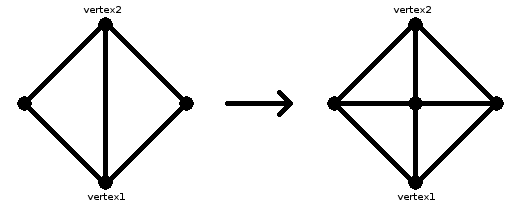
\includegraphics[scale=0.55]{img/cutEdge.png}
							\caption{Principe de la méthode cutEdge}
						\end{center}
					\end{figure}
					
				\subsubsection{Fusion de deux arêtes}
					Il est possible de fusionner deux arêtes en une seule grâce à la fonction :
					\begin{verbatim}
						bool mergeEdge(QVector3D vertex1, QVector3D vertex2, QVector3D vertex3);
					\end{verbatim}
					S'il existe une arête entre "vertex1" et "vertex2", ainsi qu'une autre entre "vertex2" et "vertex3", alors la fonction fusionne ces deux 
					arêtes. Le principe de ce processus est de ramener un éventail de son centre vers une de ses extrémités. Donc, toutes les arêtes de 
					l'éventail de centre "vertex2" se redirigeront vers "vertex1". Il est conseillé d'utiliser cette fonction avec parcimonie, notamment en 
					vérifiant les angles entre les arêtes, car aucune vérification de recoupement de faces n'est effectué.
					\begin{figure}[H]
						\begin{center}
							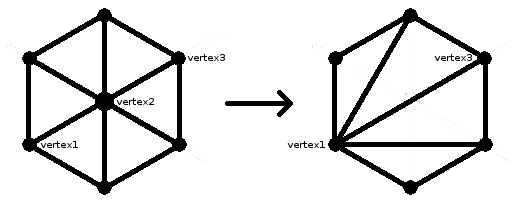
\includegraphics[scale=0.55]{img/mergeEdge.png}
							\caption{Principe de la méthode mergeEdge}
						\end{center}
					\end{figure}
					
				\subsubsection{Récupération de points}
					Il est possible de récupérer une liste de points dans une certaine zone avec :
					\begin{verbatim}
						QVector<QVector3D> getVertices(QVector3D position, float areaSize);
					\end{verbatim}
					Le but de cette fonction est de renvoyer tous les points présents dans la zone de centre "position" et de rayon "areaSize". Pour cela, 
					un parcours récursif des voisins de la face contenant le centre, couplé avec des tests de distance point à point, renvoie tous les 
					points des faces voisines tant que la distance au centre reste inférieure au rayon. Si le rayon est égal à zéro, la fonction renvoie 
					uniquement les trois points de la face contenant le centre de la zone.\\ 
					Remarque : la liste de points renvoyée contient aussi "position".
					
				\subsubsection{Récupération de voisinage}
					Il est possible de récupérer une liste de points voisins d'un certain point avec :
					\begin{verbatim}
						QVector<QVector3D> getNeighbours(QVector3D vertex, int degree);
					\end{verbatim}
					Si le point passé en paramètres existe, alors la fonction renverra, grâce à un parcours récursifs basé sur les adjacences de faces, la 
					liste des points voisins de celui-ci. Le degré de voisinage permet d'obtenir des voisins plus éloignés, ce paramètre définissant le 
					nombre de récursions à effectuer lors du parcours.
					
				\subsubsection{Récupération de normale de surface}
					Il est possible de récupérer la normale à la surface de l'objet grâce à la méthode :
					\begin{verbatim}
						QVector3D getNormal(QVector3D position);
					\end{verbatim}
					Cette méthode détecte la face contenant le point passé en paramètre, et renvoie la normale au plan contenant cette face. Si aucune face 
					n'est détectée comme contenant ce point, le vecteur renvoyé sera la direction entre le centre de l'objet et le point "position", afin 
					d'éviter les scintillements du pinceau ou autres petits décalages du curseur pouvant créer des incohérences.
					
				\subsubsection{Translation de points}
					Il est possible d'effectuer une translation sur un ou plusieurs points à l'aide des fonctions :
					\begin{verbatim}
						void moveVertex(QVector3D vertex, QVector3D move);
						void moveVertex(int index, QVector3D move);
						void moveVertices(QVector<QVector3D> vertices, QVector3D move);
					\end{verbatim}
					Ces trois fonctions permettent au développeur d'effectuer des translations sur un ou plusieurs points, selon un vecteur passé en 
					paramètres ("move").
					
				\subsubsection{Les accesseurs}
					La classe Mesh contient également certains accesseurs utiles :
					\begin{verbatim}
						QVector3D getCenter() const;
						void setCenter(QVector3D center);

						QVector3D getCoords(int index) const;
						void setCoords(QVector3D vertex, QVector3D coord);
						void setCoords(int index, QVector3D coord);

						int getEdgeCount() const;
						int getVertexCount() const;
						int getFaceCount() const;
					\end{verbatim}
					Avec ces accesseurs, nous pouvons récupérer ou déplacer des points du maillage directement (y compris le centre de l'objet), ainsi que 
					connaitres des informations utiles telles que le nombre total de points, demi-arêtes ou faces.
				
			\subsection{Les méthodes de la classe MeshRenderer}
				\label{renderer-dev}
				\subsubsection{Dessin de l'objet}
					On effectue le rendu OpenGL avec la méthode suivante :
					\begin{verbatim}
						void paintGL();
					\end{verbatim}
					Cette méthode transmet à la carte graphique (donc le GPU), les buffers nécessaires au rendu OpenGL de l'objet. Il existe trois buffers : 
					les points, les normales et les indices. Nous avons choisi de passer par un buffer d'indices afin d'améliorer les performances (un 
					entier pour chaque point de chaque triangle au lieu de répéter trois flottants pour chaque points et trois de plus pour chaque normale).
					
				\subsubsection{Synchronisation des buffers}
					Il est parfois nécessaire d'actualiser ou non les buffer objects :
					\begin{verbatim}
						void update();
					\end{verbatim}
					Cette fonction permet d'actualiser les buffers. En effet, avec les modifications sur les maillages rendues possibles, il est souvent 
					nécessaire de resynchroniser les buffers avec le maillage existant. Ce processus a été séparé du processus de rendu afin de permettre de 
					changer les options de rendus sans recalculer la synchronisation qui n'est nécessaire que si le maillage est modifié.
				
			\subsection{Les méthodes de la classe MeshProcessing}
				\label{processing-dev}
				\subsubsection{Subdivision}
					Nous avons mis en place deux types de subdivision :
					\begin{verbatim}
						static void subdivide(Mesh *mesh);
						static bool subdivideAuto(Mesh *mesh, float maxEdgeLength);
					\end{verbatim}
					Ces deux processus de subdivision permettent de raffiner le maillage dans son intégralité.\\
					La première subdivision crée pour chaque face un triangle à l'aide des milieux de chaque arête de celle-ci. Un schéma est disponible en 
					annexe (cf page \pageref{fig:subdivide}). Celle-ci étant intimement liée à la structure interne des maillages, il est nécessaire de la 
					redéfinir si l'on décide de changer cette structure.\\
					La seconde méthode est paramétrable. En effet, le paramètre "maxEdgeLength" permet de ne couper que les arêtes dépassant cette taille. 
					Un booléen atteste de la modification ou non du maillage. Le processus utilisé est celui de la méthode "cutEdge" de la classe 
					\textbf{Mesh} (cf page \pageref{mesh-dev}).
					
				\subsubsection{Décimation}
					Nous avons mis en place deux types de décimation :
					\begin{verbatim}
						static void decimate(Mesh *mesh);
						static bool decimateAuto(Mesh *mesh, float minEdgeLength);
					\end{verbatim}
					Ces deux processus de décimation permettent de simplifier le maillage dans son intégralité.\\
					La première décimation fusionne chaque ensemble de quatre faces (cf schéma de subdivision page \pageref{fig:subdivide}) en une seule, si 
					et seulement si ces faces ont des angles dièdres inférieurs à une certaine valeur (ici 22.5 degrés mais paramétrable dans l'avenir). Les 
					faces déjà visitées sont enregistrées pendant le processus afin de ne pas faire plusieurs passes en une seule fois.\\
					La seconde méthode est paramétrable. En effet, le paramètre "minEdgeLength" permet de ne fusionner que les arêtes plus courtes que cette 
					taille. Un booléen atteste de la modification ou non du maillage.\\
					Le processus utilisé pour les deux méthodes est celui de la méthode "mergeEdge" de la classe \textbf{Mesh} (cf page \pageref{mesh-dev}).
				
			\subsection{Les méthodes de la classe MeshTool}
				\label{tool-dev}
				\subsubsection{Les outils de sculpture}
					Comme expliqué précédemment (cf page \pageref{tool-cdc}), nous avons plusieurs outils de sculpture présents. Pour chacun d'entre eux, 
					il existera une unique méthode, dans la classe MeshTool, définissant son action :
					\begin{verbatim}
						void gtmove(Mesh *mesh, QVector3D move);
						void gtrotate(Mesh *mesh, QVector3D move);
						void gtscale(Mesh *mesh, QVector3D move);

						void ltadd(Mesh *mesh, QPoint last_position, float brushSize, float strength, Qt::KeyboardModifiers modifiers);
						void ltinflate(Mesh *mesh, QPoint last_position, float brushSize, float strength, Qt::KeyboardModifiers modifiers);
						void ltmove(Mesh *mesh, QPoint last_position, QVector3D move, float brushSize);
						void ltpinch(Mesh *mesh, QPoint last_position, float brushSize, float strength, Qt::KeyboardModifiers modifiers);
						void ltsmooth(Mesh *mesh, QPoint last_position, float brushSize, float strength, Qt::KeyboardModifiers modifiers);
					\end{verbatim}

					Pour chaque outil, les paramètres diffèrent légèrement. En effet, nous pouvons retrouver le maillage de l'objet sélectionné "mesh",  un vecteur de déplacement "move" (dans le 
					repère scène ou déplacement de souris), la position du curseur "last\_position", la taille de la zone d'action "brushSize", la force de 
					l'outil "strenght" (force d'attraction de la matière : Plus la force est fort, plus la modification par l'outil va etre significative), ou encore des KeyboardModifiers afin d'augmenter les possibilités de nos outils. 
					Mais comment fonctionnent ces outils ?\\\\
					\textbf{Remarque :} un Brush, cité ci-dessous, correspond à la zone circulaire de centre "last\_position" (en réalité on utilise par la 
					suite le point d'impact du curseur sur l'objet, donc des coordonnées dans le repère scène) et de rayon "brushSize". Ce brush permet de définir les sommets contenus dans cette zone où l'outil va être appliqué.
					\begin{itemize}
						\item \textbf{GTMove :} Translation par le vecteur "move" de chacun des points de l'objet.
						\item \textbf{GTRotate :} Rotation selon les composantes du vecteur "move" de chacun des points de l'objet, en prenant comme origine 
						du repère de rotation le centre de celui-ci.
						\item \textbf{GTScale :} Homothétie de l'objet selon le déplacement en ordonnées du vecteur "move", en prenant comme origine le 
						centre de l'objet.
						\item \textbf{LTAdd :} Translation de tous les points contenus dans le Brush selon la normale à la face touchée par le curseur, 
						pondérée par le paramètre "strenght". La touche Shift inverse la normale et permet donc de creuser.
						\item \textbf{LTSmooth :} Translation de chaque point contenu dans le Brush dans la direction des coordonnées moyennes de ses 
						voisins immédiats, pondérée par "strenght". La touche Shift augmente la force d'un facteur 20.
						\item \textbf{LTMove :} Translation de tous les points contenus dans le Brush selon le vecteur "move" (défini dans le repère scène).
						\item \textbf{LTInflate :} Translation de chaque point contenu dans le brush selon un vecteur défini par la normale de surface et la 
						distance entre le point et le centre du Brush. Ce vecteur est une addition du vecteur normal et de la composante plane (sur le Brush)
						du vecteur allant du centre du Brush vers le point. Ce qui a pour effet de créer un gonflement de la matière, puisque les directions
						des translations forment une bulle. La touche Shift permet d'inverser la normale et donc de creuser.
						\item \textbf{LTPinch :} Translation de chaque point contenu dans le brush selon un vecteur défini par la normale de surface et la 
						distance entre le point et le centre du Brush. Ce vecteur est une soustraction entre le vecteur normal et la composante plane (sur le
						Brush) du vecteur allant du centre du Brush vers le point. Ce qui a pour effet de créer un pincement de la matière, puisque les 
						directions des translations forment l'inverse d'une bulle. La touche Shift permet d'inverser la normale et donc de creuser.
					\end{itemize}
					\textbf{Remarque :} Les outils LTSmooth, LTMove, LTInflate et LTPinch pondèrent leurs translations par un coefficient de distance entre 
					le point translaté et le centre du Brush, de sorte que le déplacement décroisse avec la distance.
					\begin{figure}[H]
						\begin{center}
							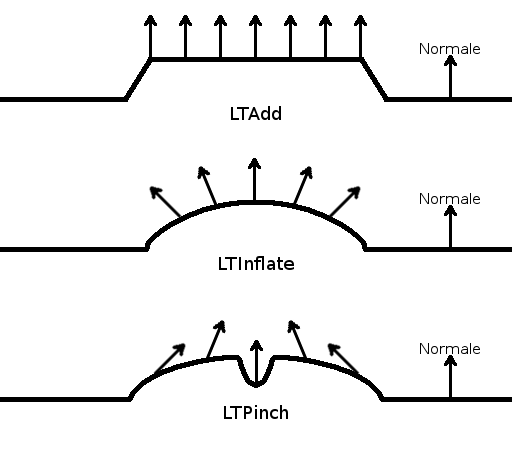
\includegraphics[scale=0.5]{img/tool-dev.png}
							\caption{Translations par les outils de sculpture}
						\end{center}
					\end{figure}
					
				\subsubsection{Les outils spéciaux}
					De nouveaux outils, nommés ici "spéciaux", ont été développés suite à la proposition de notre encadrant :
					\begin{verbatim}
						void subdivideAuto(Mesh *mesh, QPoint last_position, float brushSize);
						void decimateAuto(Mesh *mesh, QPoint last_position, float brushSize);
					\end{verbatim}
					Ces deux outils sont en fait une subdivision ou une décimation, mais uniquement locale. Nous pouvons les utiliser soit seul, soit 
					conjointement à un des outils de sculpture. Ce sont en fait des processus paramétrés, d'où le "Auto" rappelant les méthodes de la classe 
					\textbf{MeshProcessing} (cf page \pageref{processing-dev}). En réalité, le processus est similaire, sauf qu'ici le paramètre de longueur 
					d'arête est calculé grâce à une moyenne des longueurs d'arêtes contenues dans la zone d'action. Les fonctions utilisées sont également 
					"cutEdge" et "mergeEdge" de la classe \textbf{Mesh} (cf page \pageref{mesh-dev});
				
			\subsection{Les méthodes de la classe MeshManager}
				\label{manager-dev}
				\subsubsection{Dessin et synchronisation}
					On effectue le rendu OpenGL et la synchronisation des buffers à l'aide de ces fonctions :
					\begin{verbatim}
						void paintGL(int activeMesh);
						void updateMesh(int index);
						void updateLastMesh();
					\end{verbatim}
					Cette classe permet facilement de faire appel à tous les objets itérativement, et offre également quelques options. En effet, le 
					paramètre "activeMesh" permet le rendu du maillage actif d'un couleur différente des autres par exemple. De même, nous pouvons choisir 
					quel maillage nous avons besoin de mettre à jour.
					
				\subsubsection{Ajout et suppression}
					Puisque le MeshManager est un conteneur, il est possible d'ajouter ou de supprimer un ou plusieurs maillages :
					\begin{verbatim}
						void addMesh(Mesh *mesh);
						void removeMesh(Mesh *mesh);
						void clear();
					\end{verbatim}
					Ces fonctions d'ajout et suppression permettent de ne pas gérer nous même les suppressions d'objet de la mémoire, puisque le manager 
					s'en occupe. Ainsi, la programmation s'en retrouve moins compliquée.
		
		\section{...}
			% TODO : diagrammes, problèmes et solutions, précisions (PEU DE CODE, PAS TROP UTILE SUR L'INTERFACE)...etc
			% TODO : Yannick : interface
			% TODO : Cécile si t'as des trucs à dire hors API
			\subsection{...}

%==========================================================================================================================================================
	\chapter{Manuel}
		Ce chapitre détaille tout ce qui concerne l'utilisation de l'application, autant pour les utilisateurs que les développeurs souhaitant étendre les 
		possibilités du logiciel.
		
		\section{Utilisateur}

			% TODO : image de l'interface avec explications, raccourcis clavier, menus...etc
			L'interface se d\'ecompose en 4 parties. Nous avons donc une partie qui agira sur la figure (le panel \`a droite), une partie qui listera les mod\`eles  pr\'esent dans la sc\`ene (le panel \`a droite), une partie qui agira sur la sc\`ene (le panel en haut), et enfin une fen\^etre au centre qui sera le rendu de la sc\`ene.\\
			Nous aurons donc une interface du type :\\ mettre la figue 
			

			% TODO : Yannick : image de l'interface avec explications, raccourcis clavier, menus...etc


		\section{Développeur}
			Toute personne avec des bases de programmation pourra étendre les fonctionnalités de celle-ci grâce à notre API. Les seuls prérequis seront 
			d'installer QtCreator et d'avoir les librairies Glut pour OpenGL.
			
			\subsection{Ajout d'un maillage modèle}
				Il est possible d'ajouter un maillage modèle afin d'enrichir les objets de base proposés à l'utilisateur.\\
				Pour cela, il est nécessaire d'ajouter plusieurs choses :
				\begin{itemize}
					\item Une fonction de génération du maillage dans la classe \textbf{Mesh}
					\item Un bouton ou une entrée de menu pour créer le modèle dans l'interface
					\item Des widgets (s'ils n'existent pas encore) pour les paramètres de génération
					\item Une fonction de mise à jour du maillage en temps réel
				\end{itemize}
				
				\subsubsection{Fonction de génération}
					Il est nécessaire d'ajouter cette fonction dans la classe \textbf{Mesh}. Nous conseillons, pour la clarté, de placer sa déclaration dans 
					"Mesh.h", sous les méthodes existantes de type :
					\begin{verbatim}
						void makeCube(float width, float height, float depth, int discretization);
					\end{verbatim}
					Toujours pour la facilité d'appréhension du code, nous conseillons de créer un nouveau fichier "make\textit{Polygon}.cpp" contenant la 
					définition de la fonction :
					\begin{verbatim}
						#include "Mesh.h"

						void Mesh::makeCube(float width, float height, float depth, int discretization) {
						    this->clear();
							
						    ...
							
						    this->TEST();
						}
					\end{verbatim}
					Il faut donc absolument inclure "Mesh.h", et surtout ne pas oublier d'utiliser la fonction clear(), qui permet de régénérer le maillage à
					chaque changement de paramètre. Une fonction TEST() est également disponible pour vérifier l'intégrité du maillage (à utiliser à la fin 
					de la fonction make\textit{Polygon}). Dans le corps de cette méthode, il est conseillé d'utiliser la méthode addFace (cf page 
					\pageref{mesh-dev}) pour chaque facette du maillage. Vous pourrez bien sûr prendre exemple des fonctions déjà implémentées.
					
				\subsubsection{Bouton, menu et widgets}
					%TODO : Yannick
					
				\subsubsection{Fonction de mise à jour}
					Il est nécessaire d'ajouter cette fonction dans la classe \textbf{MainWindow}. Nous conseillons de placer sa déclaration dans 
					"MainWindow.h", sous les méthodes existantes de type :
					\begin{verbatim}
						void updateCube();
					\end{verbatim}
					Il suffit ensuite de placer sa définition dans "MainWindow.cpp", selon l'exemple des méthodes déjà implémentées. Cette fonction est 
					obligatoire pour la génération (et régénération) du maillage.
				
			\subsection{Ajout d'un outil}
				Il est possible d'ajouter un outil afin d'enrichir les actions de sculpture proposées à l'utilisateur.\\
				Pour cela, il est nécessaire d'ajouter plusieurs choses :
				\begin{itemize}
					\item Un type d'outil dans l'énumération \textbf{TOOL}
					\item Une fonction d'action de l'outil dans la classe \textbf{MeshTool}
					\item Un bouton pour utiliser l'outil dans l'interface
					\item Une entrée dans la méthode "mouseMoveEvent" de la classe \textbf{GLWidget}
				\end{itemize}
				
				\subsubsection{Type d'outil et fonction d'action}
					Il est nécessaire d'ajouter le type de votre outil dans l'énumération "TOOL", déclarée dans le fichier "MeshTool.h". Pour la clarté, il 
					est conseillé de respecter la convention de nom expliquée en commentaire au dessus de l'énumération.\\
					Vous devez ensuite créer une méthode d'action. Nous vous conseillons de vous imprégner de la partie \textbf{Développement} (cf page 
					\pageref{tool-dev}) pour choisir les paramètres adéquats. Il suffit de la déclarer dans le fichier "MeshTool.h", sous les méthodes 
					existantes de type :
					\begin{verbatim}
						void gtmove(Mesh *mesh, QVector3D move);
					\end{verbatim}
					La déclaration se place dans le fichier "MeshTool.cpp". Il est encore une fois conseillé de bien comprendre la partie 
					\textbf{Développement} (cf page \pageref{tool-dev}) afin de créer l'effet désiré. De même, les fonctions déjà présentes pourront servir 
					d'exemple. Les fonctions du fichier "functions.h" sont également très utiles.
					
				\subsubsection{Bouton}
					%TODO : Yannick
					
				\subsubsection{Une réaction à l'évènement souris}
					La fonction "mouseMoveEvent" de la classe \textbf{GLWidget} s'occupe de gérer les outils à l'aide d'un switch. Vous devrez donc ajouter 
					une entrée dans cette fonction afin de pouvoir utiliser votre outil. Seul le fichier "GLWidget.cpp" est utile ici :
					\begin{verbatim}
						void GLWidget::mouseMoveEvent(QMouseEvent *event) {
						    ...
						    switch(activeTool) {
						        case GTSCALE:
						            m_tool.gtscale(m_manager.getMesh(activeMesh), QVector3D(0, dy, 0));
						            break;
						    ...
						    }
						    ...
						}
					\end{verbatim}
					Nous vous conseillons de vous imprégner de la partie \textbf{Développement} (cf page \pageref{tool-dev} et \pageref{glwidget-dev}) pour 
					choisir les paramètres adéquats.
				
			\subsection{Pour aller plus loin...}
				Si un développeur souhaite modifier plus profondément l'application, il faudra pour cela se référer à la partie \textbf{Développement} (cf 
				page \pageref{dev}), notamment les explications détaillant l'\textbf{API} (cf page \pageref{api-dev}).

%==========================================================================================================================================================
	\chapter{Post-Mortem}
		Cette section liste toutes les étapes de la conception que nous n'avons pas réalisées (selon notre ordre de priorités), ainsi que toutes les 
		améliorations auxquelles nous avons pensé lors de la phase de développement.
		
		\section{Fonctionnalités non implémentées}
			Nous avions, lors de la conception de ce projet, prévu nombre de fonctionnalités. Malheureusement, ce projet ayant une durée de 
			développement limitée à quatre semaines, nous n'avons pas pu toutes les mettre en place.\\
			Voici une liste non exhaustive de certaines fonctionnalités que nous voulions :
			\begin{itemize}
				\item Possibilité de créer et placer plusieurs lumières, ou déplacer l'existante, afin de créer une illumination personnalisée de notre 
				scène.
				\item Possibilité de créer ou utiliser différents matériaux ou shader pour nos objets.
				\item Possibilité de peindre nos objets avec différentes couleurs (un color-picker aurait pu être présent), ainsi que leur appliquer 
				une texture de notre choix.
				\item Implémenter un "mode miroir" pour la sculpture. Ce mode permettrait à l'utilisateur de sculpter l'objet symétriquement, en 
				n'agissant que sur un côté de celui-ci. Nous aurions voulu pouvoir implémenter une symétrie en abscisse, en ordonnées ou en profondeur, 
				ainsi qu'une symétrie centrale permettant facilement de modeler des cercles parfaits.
				\item Implémenter des outils d'union, différence et intersection d'objets entre eux.
				\item Permettre de passer d'une représentation surfacique à une représentation volumique et inversément.
				\item Permettre l'affichage d'une grille (deux ou trois dimensions), ainsi que les repères scène et objet.
				%TODO : si on ne fait pas undo/redo et importer/exporter, le noter ici
			\end{itemize}
			
		\section{Améliorations réalisables}
			Comme pour tout projet, la conception n'offre pas toujours une liste exhaustive des fonctionnalités futures, étant donné que nous pouvons 
			toujours améliorer notre programme selon les possibilités offertes par le développement de celui-ci. Ainsi, nous avons quelques suggestions 
			d'améliorations pour notre logiciel, dans le cadre d'une éventuelle future reprise de son développement :
			\begin{itemize}
				\item Optimisation : beaucoup de nos algorithmes pourraient être améliorés, notamment les comparaisons de points de par la surcouche de 
				l'API qui se déroulent en O(n) et pourraient l'être en O(1) avec par exemple des fonctions de hachage. D'autres, plus coûteux, 
				nécessiteraient une recherche approfondie pour améliorer les performances.
				\item Contenu : notre logiciel ne propose que cinq outils et cinq maillages prédéfinis, un aspect qui pourrait facilement être enrichi 
				avec plus de temps.
				\item Maillage : il serait utile de mettre en place bon nombre de fonctions de vérifications de maillage, notamment les recoupements 
				de triangles.
				\item Autre : les fonctions de subdivision et décimation mériteraient sûrement d'être améliorées, notamment la décimation globale qui ne
				fait pas exactement l'inverse de la subdivision. De plus, les rotations ne s'effectue actuellement que par rapport au déplacement souris,
				et ne prennent donc pas en compte l'angle de vue actuel.
				%TODO : si d'autres idées, ne pas hésiter à ajouter
			\end{itemize}

%==========================================================================================================================================================
	\appendix
	\chapter{}
		Dans cette partie seront placés les éléments trop volumineux pour être inclus directement dans le texte, tels que les images ou graphiques.\\
		
		\section{Diagramme de Gantt}
			Les diagrammes sont fournis page \pageref{fig:gantt}.
			
		\section{Comparatif de performances}
			Le graphique est situé page \pageref{fig:analyse}.
			
		\section{Diagramme de Classes}
			Le diagramme est fournis page \pageref{fig:diagClass}.
			
		\section*{}
			\begin{figure}
				\vspace{-3,5cm} \hspace{-4,5cm} 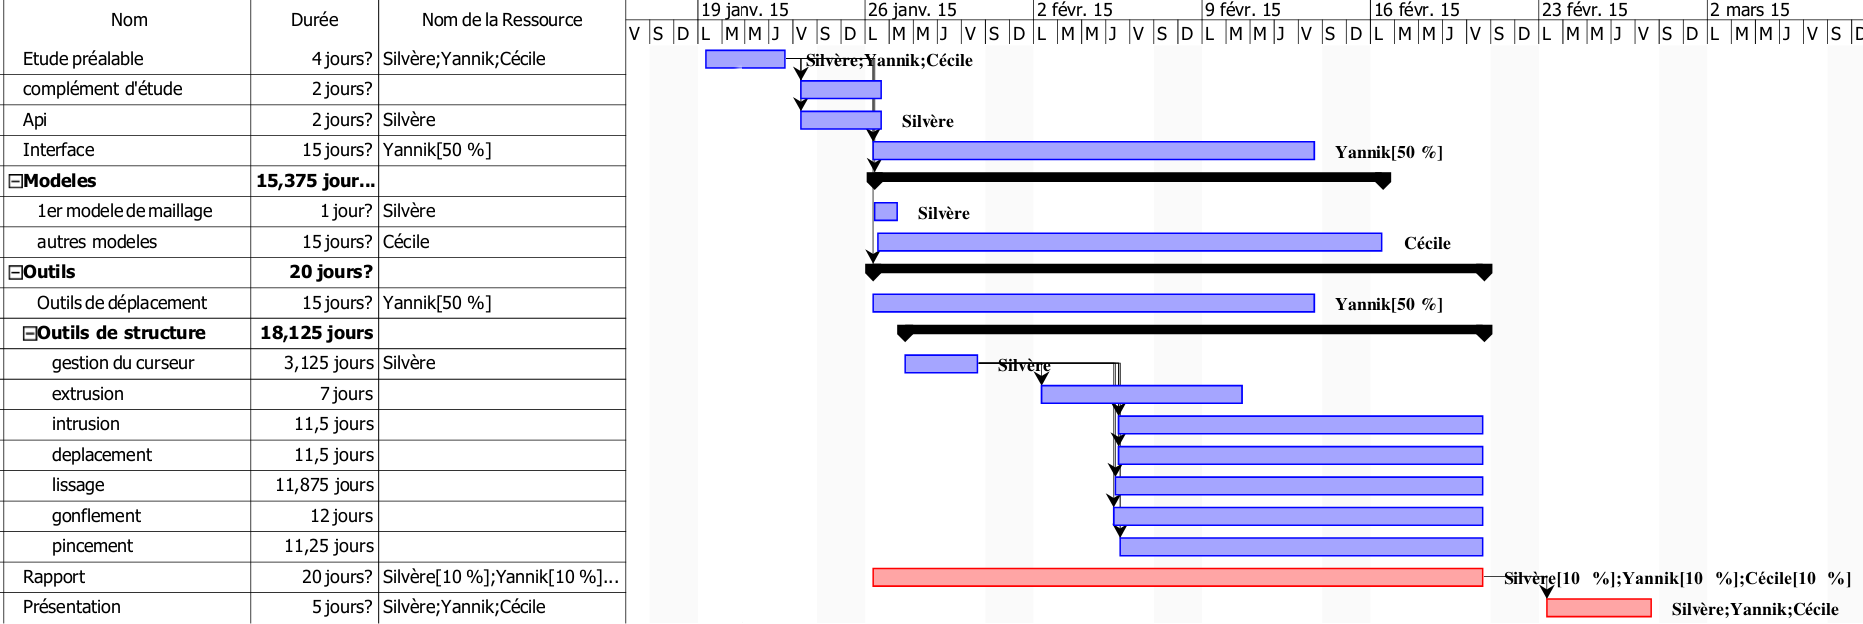
\includegraphics[scale=0.6]{img/Gantt1.png}
				\vspace{-3,5cm} \hspace{-4,5cm} 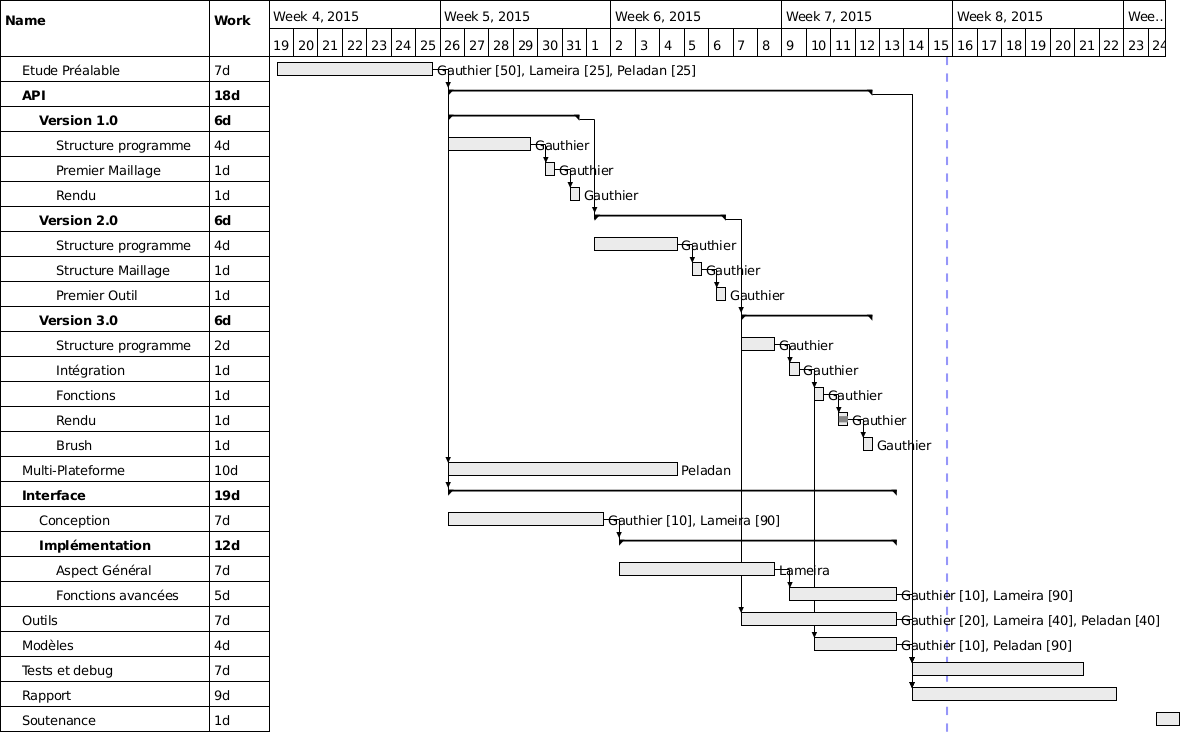
\includegraphics[scale=0.6]{img/Gantt2.png}
				\label{fig:gantt}
				\vspace{-0,5cm} \caption{Diagrammes de Gantt prédictif et final}
			\end{figure}
			
			\begin{figure}
				\begin{center}
					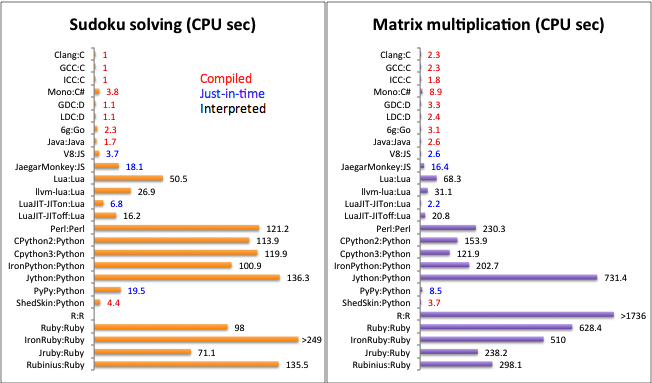
\includegraphics[scale=0.5]{img/AnalyseLangage1.png}
					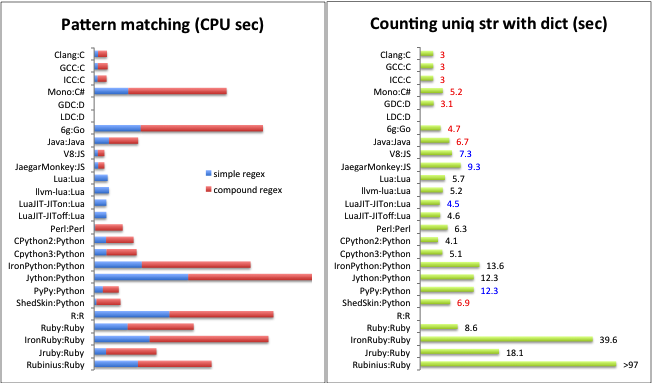
\includegraphics[scale=0.5]{img/AnalyseLangage2.png} 
				\end{center}
				\label{fig:analyse}
				\caption{Comparaisons de performances de divers langages dans des cas donnés}
				Source : \url{http://attractivechaos.wordpress.com/2011/06/22/my-programming-language-benchmark-analyses/}
			\end{figure}
			
			\begin{figure}
					\hspace{-2,75cm}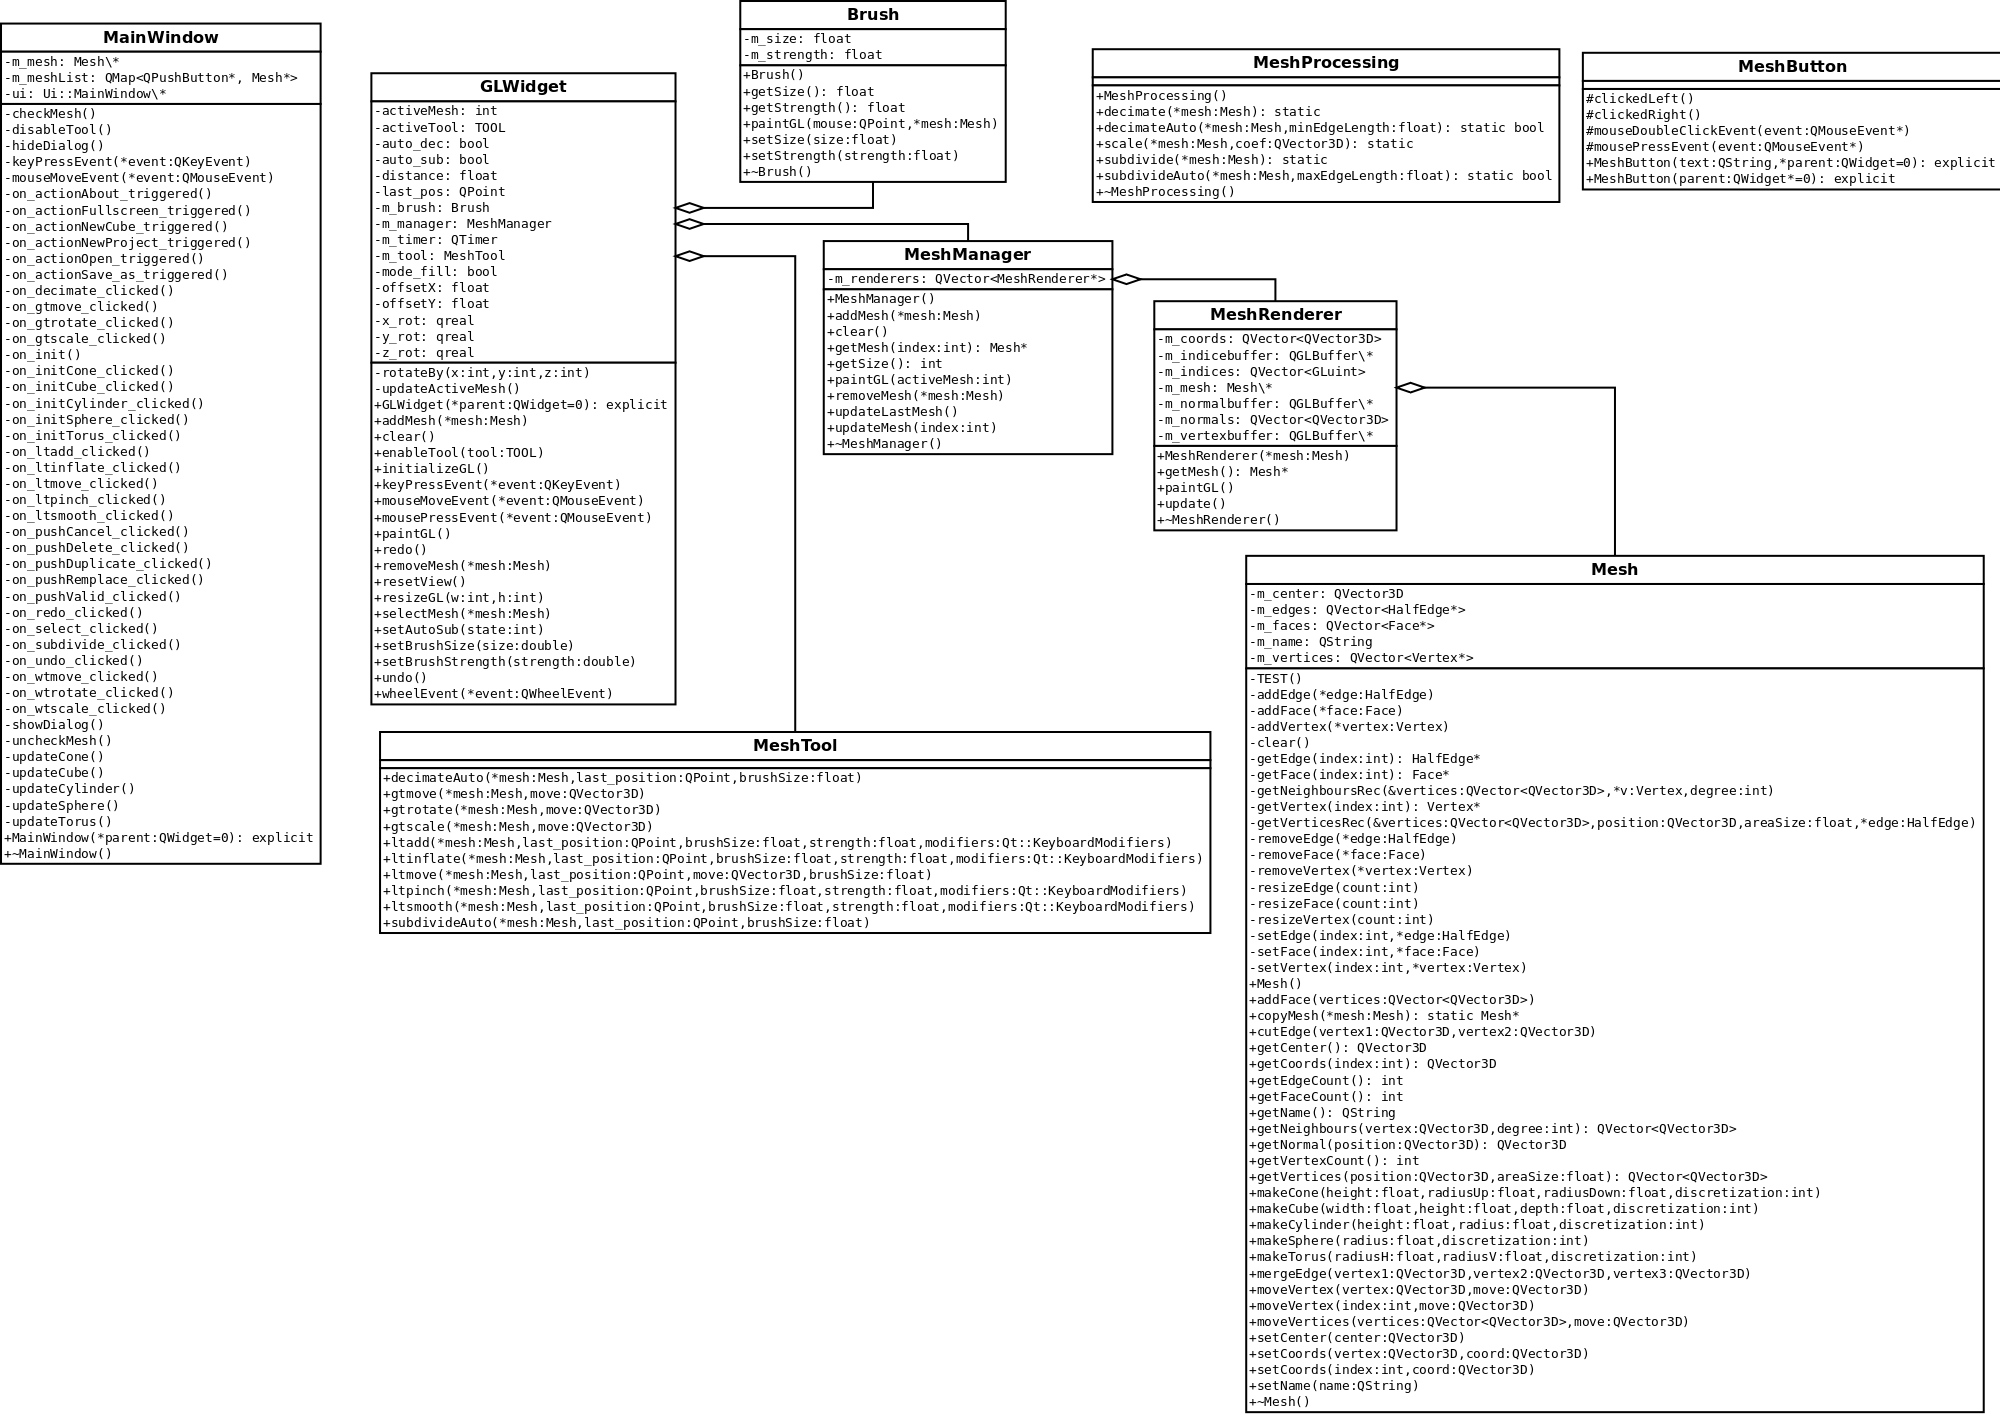
\includegraphics{img/diagClass.png}
				\label{fig:diagClass}
				\caption{Diagramme de classes de notre API}
			\end{figure}
			
			\begin{figure}
				\hspace{-3cm}
\includegraphics[scale=0.5]{img/subdivide.png}
				\label{fig:subdivide}
				\caption{Schéma de subdivision globale}
			\end{figure}

\end{document}
